%	Größen in TeX:
%		mm, cm, ... uninteressant
%		1 em = Schriftgröße, ursprünglich
%		1 ex = Schriftgröße, skaliert auf die Box in welcher sich die Schrift befindet
%		1 pt = ein Pixel nur kann man nicht von echten Pixeln wie auf einem Bildschirm sprechen
%		\textwidth, \paperwidth, ...

\documentclass[11pt,toc,multi=tcblisting]{article}
\renewcommand{\familydefault}{\sfdefault}
\setcounter{secnumdepth}{6}

\usepackage[left=2cm,right=2cm]{geometry}
%\usepackage[document]{ragged2e} % Damit alles: Links aligned (der linkeste Punkt eines jeden Buchstaben ist auf einer Linie für alle zeilen) und so viel Platz nach rechts ausnutzt, wie möglich (nein, macht TeX nicht standardmäßig); muss man nicht für das gesamte Dokument machen (wie hier), geht auch per \raggedright oder \RaggedRight für/vor Paragraphen; gibt auch Umgebungen für rechtsbündigen Text https://de.overleaf.com/learn/latex/Text_alignment
\usepackage[dvipsnames]{xcolor}
\usepackage{booktabs,array}
\usepackage[author={Hendrik Theede}]{pdfcomment}
\usepackage{tabularx}


\usepackage[utf8]{inputenc}
\usepackage[T1]{fontenc}

\usepackage{inconsolata}
\usepackage[htt]{hyphenat}
\usepackage{listings}
% Note: lstset does not allow unnecessary linebreaks
\lstdefinestyle{texstyle}{
	% Colors
	backgroundcolor=\color{white},
    commentstyle=\color{SeaGreen},
    keywordstyle=\color{Magenta},
    numberstyle=\tiny\color{red},
    stringstyle=\color{Fuchsia},
    basicstyle=\ttfamily\footnotesize\color{black},
	% Linebreaks and Whitespace
    breaklines=true,% Sagt: Bei benötigtem Zeilenumbruch gehen wir in eine neue Zeile
	%breakatwhitespace=true,   
	showspaces=false,                
    showstringspaces=false,
    showtabs=false,
	frame=single,
	xleftmargin=13pt,
	aboveskip=13pt,
	%
	% Indentation
	tabsize=2,
	breakindent=13pt,
    framesep=2mm,
    framerule=0mm,
    abovecaptionskip=5mm,
    aboveskip=\baselineskip,
    belowskip=\baselineskip,
	lineskip=1ex,
	postbreak=\raisebox{0ex}[0ex][0ex]{\tiny\tiny$\hookrightarrow$}, % \rule[Offset (Y)]{Breite}{Höhe}, hiermit nochmal rumspielen. 
	% Captions
    captionpos=b,                    
    keepspaces=true,    
	% Linenumbers
    numbers=left,      % where to place numbers
    numbersep=0pt,     % distance to the (here) left   
    % Encodings
	inputencoding=utf8,
	extendedchars=true,
	literate=
		{ä}{{\"a}}1 {ö}{{\"o}}1 {ü}{{\"u}}1 {Ä}{{\"A}}1 {Ö}{{\"O}}1 {Ü}{{\"U}}1
}
\lstset{style=texstyle}



%%%%%%% Vorsicht, evtl Redundanzen im Code!!!
%%% Benötigt noch intensivere Dokumentation
%%% Siehe Package auf CTAN
\usepackage[many]{tcolorbox}
\tcbuselibrary{skins,breakable,listings}
%https://tex.stackexchange.com/questions/530859/add-option-to-point-to-code-file-in-tcblisting-environment 
\newcounter{texlst}
\newtcbinputlisting[use counter=texlst]{\commoncode}[3][]{%
        enhanced,
		noparskip,
		breakable,
		colback=gray,
		opacitybacktitle=.8,%
        fonttitle=\bfseries,
        %title after break={\centering\footnotesize\itshape\strut\lstlistingname~\thelstlisting~--~continued},%
        listing only,
		listing options={style=texstyle, xleftmargin=-1mm},
		after upper={\centering\strut\TeX{} Code~\thetcbcounter:~#2},
        frame hidden,
		arc=13pt,
		outer arc=13pt,
		boxrule=2pt,
        listing file = {#3}, #1
}


\usepackage{minted}
\usepackage{graphicx}
\usepackage{pdfpages} 
\usepackage{caption}
\usepackage{subcaption}




\usepackage[english,ngerman]{babel}
\usepackage[english=british]{csquotes}

\usepackage{tikz}
\usetikzlibrary{calc,positioning}
\usepackage{pgfplots}
\usepackage[nottoc]{tocbibind}
\usepackage{amsmath}

% Danke an https://tex.stackexchange.com/questions/14342/verbatim-environment-that-can-break-long-lines
\usepackage{fancyvrb}
\usepackage{fvextra}
% !!! Funktioniert nur mit ASCII-Zeichen (nicht mit deutschen Umlauten ä,ö,ü(,ß))

\usepackage{natbib}
\bibliographystyle{agsm}

%%% Uni-HRO relevantes
%%% TeX-relevant (siehe: titlepage.tex)
\author{Hendrik Theede}
\date{02.12.2025}
\title{Automatische Sprachübersetzung von \LaTeX{}-Dokumenten}
\def\matrikelnummer{221201256}
\newcommand{\supervisor}{Prof.\ Dr.\ rer.\ nat.\ habil. Clemens H. Cap}					% Betreuer
\newcommand{\ief}{Fakultät für Elektrotechnik und Informatik}							% Fakultaet
\definecolor{colorscheme}{cmyk}{0.90, 0.30, 0.00, 0.00} 								% Farbschema der Fakultaet; Siehe Corp. Design
\newcommand{\iuk}{Lehrstuhl für Informations- und Kommunikationsdienste}				% Institut



%%% "Deutsche Sprache"-relevant
\renewcommand*\contentsname{\hypertarget{toc}{Inhaltsverzeichnis}} % cannot contain \par (and thus: newlines)
\renewcommand*\refname{Literaturverzeichnis} % can contain \par (and thus: newlines)
\renewcommand*\figurename{Abbildung}



% Muss ans Ende, weil sonst übernimmt ein Biber aus der Bibliothek
\usepackage{hyperref}					% TeX!	
\hypersetup{
		linktoc=all,
		allcolors=black,
		colorlinks=true, % Für offizielle Releases das % vorne wegnehmen. Ersetzt die Boxen um Links durch die eigentlichen Farben
		linkcolor=black,
		urlbordercolor={1 0 0},
		urlcolor=blue, 
		citecolor=magenta,
		breaklinks=true,
		pdftitle=Abschlussarbeit,
		pdfauthor=Hendrik Theede,
		pdfsubject=Matrikelnummer 221201256,
		pageanchor,
		backref,
}

\begin{document}

\makeatletter % um \@author und co zu nutzen
\thispagestyle{empty}

\begin{figure}[h!]
\begin{tikzpicture}[remember picture,overlay,shift=(current page.south west)] 
	\begin{scope}
		% Koordinaten für Titel...
		\coordinate (A) at (3.7cm,20cm);
		% ... und Angaben
		\coordinate (B) at (3.7cm,3cm);
		
		% Uni-Logo
		\node [right] at (2cm,25cm) {
\includegraphics[width=12cm]{pictures/UNIHRO_LOGO_2025.pdf}};
		
		% Rahmen
		\draw[line width=2pt,colorscheme,rounded corners=2ex] (0cm,0cm) +(2cm,0cm) --(2cm,23.5cm) -- (19cm,23.5cm) -- (19cm,0cm);
		
		% Titel
		\node at (A) [below right] {\parbox{.85\textwidth}{\noindent\bfseries\sffamily{\Huge\raggedright \textcolor{colorscheme}{\@title}\par}}};
		
		% Angaben
		\node at (B) [above right] {\parbox{.85\textwidth}{
				\begin{tabular}{ll}
					Name: & \Large\@author				\\[2pt]
					Matrikelnummer: & \matrikelnummer					\\[1ex]
					Abgabedatum: & \@date				\\[5ex]
					Betreuer und Gutachter: & \supervisor  		\\[2pt]
					& Universität Rostock						\\[2pt]
					& \ief										\\
				\end{tabular}
			}
		};
		
		\fill[colorscheme] (0cm,0cm) +(2cm,0cm) rectangle (19cm,2cm);
		\path (3.7cm,1.5cm) [right,white] node{\Large\sffamily\textbf{\Large{Bachelorarbeit}} \small{am \iuk}};
		\path (3.7cm,.8cm) [right,white] node{\Large\sffamily\textbf{\ief}};
	\end{scope}
\end{tikzpicture}
\end{figure}
\makeatother



\pagenumbering{Roman}
\setcounter{page}{0}
\newpage
\newpage
\section*{Abstrakt}
placeholder
\newpage
\tableofcontents
\newpage
\pagenumbering{arabic}

\begingroup
\hypersetup{hidelinks,pdfborder={0 0 1},allbordercolors=magenta}% Hat länger gedauert, als mir lieb ist. sagt TeX: innerhalb dieser Gruppe sollen links nicht farbig sein. würde zuerst auch implizieren, dass keine Rahmen in der PDF angezeigt werden sollen. Wie löst man das? Indem man manuell sagt: Wir haben einen Rahmen um Hyperrefs mit Offset X = 0, Offset Y = 0 und Stärke in Pixeln: 1 (standard)

\section{Einleitung}
Wohingegen sich die Sprachübersetzung im Web schnell auf gängige Technologien wie DeepL oder Google's Gemini zurückführen lässt, zeigt sich eine ähnliche Übersetzung von \TeX{} und \LaTeX{} Dokumenten nur in ernüchternder Weise verfolgt. Lösungsansätze zu diesem Problem existieren bereits, allerdings gehen diese oftmals Umwege und trennen die Fähigkeiten der \TeX{}-Engine nicht in jedem Fall von den Technologien, welche verwendet werden sollen, um textliche Inhalte einer menschlichen Sprache in eine Andere zu übersetzen.\\
\noindent
Wo eine naive Nutzung solcher Software bereits im Alltag schnell Schwierigkeiten aufzeigt, ist insbesondere in einem wissenschaftlichen und mathematischem Kontext eine gezielte Verwendung der dieser Technologien erstrebenswert, sodass nicht jegliche Texte unabhängig voneinander und kontextlos übersetzt werden. Andernfalls wäre es denkbar, dass das deutsche Wort \enquote{ungerade} seine Bedeutung gegenüber einer mathematischen Operation verliert (nach welcher eine Zahl modulo 2 in 1 resultiert) und als umgangssprachliches \enquote{schief} interpretiert wird und im Englischen respektiv als \enquote{odd}, bzw.\ \enquote{crooked} übersetzt werden würde. Neben einer solchen Erhaltung von Kontexten ist auch eine selbstständige Erkennung der zu übersetzenden Sprache (Originalsprache eines Dokumentes) interessant, jedoch nicht zwingend erforderlich.\\
\noindent
Weiterhin dürfen Übersetzungsprozesse selbstverständlich nicht darin enden, dass eine entstehende (bspw.) PDF entweder vollständig unlesbar wird. % TeX Syntax kaputt
Daneben sollten allerdings auch keine unlesbaren Sektionen innerhalb der jeweiligen Dokumente entstehen, die aus von Layouting-Problemen resultieren, welche sich für die Übersetzung in einige Sprachen zeigen (jedoch in einigen Fällen unvermeidbar sind).\\ 
\noindent
Wünschenswert ist neben vorigen Aspekten auch Möglichkeiten für den Endnutzer zu erlauben, sollte dieser spezielle Übersetzungen oder Kontexte für einige Wörter wünschen, welche jedoch nicht aus dem Dokument selbst hervorgehen. % Schaffe ich es in dieser Arbeit das Wort "inhärent" NICHT zu verwenden?
Außerdem sollte ein möglichst hoher Support für sowohl verschiedene menschliche Sprachen, aber auch verschiedene \LaTeX{}-Pakete gegeben sein, wobei Letzteres nur ein Bonus ist, sollten Systeme wie Ti\textit{k}Z, bzw.\ \texttt{pgfplots} oder Bib\TeX{} innerhalb \LaTeX{} (zusammen mit \TeX{}) nutzbar bleiben.% Da sich durch diese sämtliche Verhalten anderer Pakete reproduzieren ließen.
%%%%% Kurzer Reminder für die wichtigsten Tücken (aber auch 'benefits' (EN für: Vorteil)) der deutschen Sprache für nativ dieser Sprache Mächtigen, welche nicht in wissenschaftliche Arbeiten fließen sollten. 
%%%%% 
%%%%% Meist recht offensichtlich.
%%%%%
%%%%% Konjunktiv 2: Impliziert meist eine Form von "Subjekt hätte etwas tun müssen" oder "Subjekt wird etwas tun" (oder schlimmer noch passiv: "mit Subject wird etwas geschehen", hier braucht es sogar das Partizip 2). Intuitiv wird klar, dass etwas nicht stattfand. Eine Quelle von möglicher Redundanz. Modalverben stehen oft in Verbindung mit solchen Implikationen ("dürfte ich etwas", "müsste ich etwas", "könnte ich etwas"... meist: ja, theoretisch gesehen "kann" man alles. Daher nicht schreiben: "man müsste/könnte/sollte etwas [so und so] machen", sondern: "A existiert, wodurch sich B ergibt). Siehe: Konditionalsätze
%%%%% Konzessivsätze: Leicht am Konjunktiv 2 zu erkennen. "Entgegen Behauptung X, ist die Realität Y". Die Realität gehört an den Anfang und aus dieser sollte genug Information hervorgehen, dass Behauptung X nicht ausformuliert werden muss.
%%%%% 
%%%%% Implikationen: Erklärung bedürfte eigentlich einem (mir noch unbekanntem) wissenschaftlichen Teilgebiet der "Aussagentheorie". Entspringt der Modularität deutscher Substantive ("Rindfleischetikettierungsüberwachungsaufgabenübertragungsgesetz" als Beispiel. Wir beschäftigen uns mit der Rindfleischetikettierung, welche überwacht werden soll. Das "s" nach "Rindfleischetikettierung" entstammt einem implizierten Genitiv (Überwachung der Rindfleischetikettierung = Rindfleischetikettierungsüberwachung), genauso wie das "s" nach "[...]überwachung[...]" (Aufgabenübertragung (bei) der Überwachung). Letztendliches "s" vor "[...]gesetz" ist am einfachsten, da sich Gesetze immer auf etwas beziehen. "Ein Gesetz einer Sache" kann zu "Gesetz der Sache" vereinfacht werden, aus welcher der Genitiv wieder hervorgeht).  

%%%%% Konditionalsätze: 
%%%%% "Aus These X, folgt Hypothese". "Daher folgt die nächste Hypothese". (Hypothese = These, welche auf einer anderen These aufbaut. Grundlage der Mathematik)
%%%%% Formal entweder eine Bedingung in einem Nebensatz (if-else statement) oder Schlussfolgerung in einem Hauptsatz (Folgesatz, vergleichbar: Zuweisungen). 
%%%%% - Arten: Real und Irreal = Erfüllbare und nicht erfüllbare Bedingungen. 
%%%%% - meint: Solange ich atme, bin ich. (Wenn ich für immer aufhören würde zu atmen, wäre erste Bedingung nicht mehr erfüllt. Ich bin ein Mensch, daher stimmt die Aussage.)
%%%%% - meint: Gäbe es keine Luft, wäre ich nicht. (Annahme: Die Luft bleibt uns vorerst noch einatembar erhalten)
%%%%% - meint: Hätte es nie Luft gegeben, hätte es mich nie geben können. (Wir schließen den Kreis zu Konjunktiv 2 und bemerken das Plusquamperfekt).

%%%%% Plusquamperfekt: Als ich (etwas) tat, war (etwas anderes) bereits passiert. Oder Konditionalsatz mit Konjunktiv 2: Wäre (etwas) nie geschehen, hätte (Resultat) nie erscheinen können. Passiert umgangssprachlich oft "hätte ich (das und das [besser]) gemacht, hätte ich (das und das) bereits erreicht" bspw.: "Hätte ich keinen zweiten Versuch für eine Abschlussarbeit benötigt, hätte ich bereits den Studiengang beenden können. (Hier bemerkt man direkt: "beenden können" kann zu "beendet" gekürzt werden. Partizip II ist meist umgangssprachlich, da textlich nicht von Nöten).


%%%%%%%%%%%%% Versuche die deutsche wissenschaftliche Sprache verständlich zu halten:
%%%%%%%%%%%%% - Infinitiv so oft wie möglich (durch Substantivierung oder Erweiterung).
%%%%%%%%%%%%% - Reale Konditionalsätze nutzen

% Welche Arten von Fehlern können entstehen? (Was fällt einem auf, wenn man Dokumente schreibt und sich denkt: mmmmhh würde google translate das richtig übersetzen)
\section{Problemfälle}
Eine einzige, feste \TeX{}-Syntax existiert theoretisch gesehen nicht, wie ein~\hyperref[problems:advanced:catcode]{späterer Paragraph} aufzeigen wird.% So gehen in-document refs ganz gut.
Die Fähigkeit jegliche erdenkliche Zeichenkette (gegeben:\ diese ist auf einem Rechner darstellbar, siehe:~\cite{unicode}) sorgt zunächst für eine unendliche Menge an testbaren Problemen. Da es unmöglich ist eine unendliche Menge an Testfällen abzudecken, wird zunächst nur die vorgesehene \LaTeX{} (bzw.\ \TeX{}~Syntax nach~\cite{texbook}) betrachtet und die bereits rein innerhalb dieser schnellig auffallenden Fehler aufgezeigt, welche durch fälschlich übersetzte Zeichenketten entstehen könnten.\\\noindent
% reviewed: 1
% 
\subsection{Struktur}\phantomsection\label{problems:structure}% Warum Kategoriesieren?
\subsubsection{Klassifizierung}
Für spätere Testzwecke wurden die verschiedenen Problemfälle in einzelne Kategorien getrennt. Eine solche Kategorisierung ist technisch gesehen nicht zwingend, soll allerdings zur Verbesserung einer späteren Übersicht dienen. Die Einteilung konzentriert sich vorrangig auf die Komplexität des Problemes und in einer Reihenfolge, in welcher sie auch bei der Nutzung von \TeX{} für ein beliebiges Dokument auftreten könnten. 
%
% Definition: Direkte Probleme
Hierbei seien \textit{direkte Probleme} zunächst eher simple und technisch leicht zu behebende Probleme, welche sich durch ein einheitliches Vorgehen beheben lassen könnten.% Könnten muss an dieser Stelle so folgen
Zudem beschränkt man sich hier nur auf den benötigten Zugriff auf eine einzelne Datei.
%
% Definition: Indirekte Probleme und Zusammenfassung zu "simplen Problemen"
\textit{Indirekte Probleme} formen potentielle Schwierigkeiten, da sie einen Zugriff auf weitere Dateien benötigen, da sie von einer Ausgangsdatei referenziert werden. Technisch gesehen sind sie jedoch auch durch einheitliche Paradigma zu bewältigen. Daher werden sie im Kapitel~\ref{problems:simple} zusammengefasst und fortan als \enquote{simple Probleme} bezeichnet.
%
% Definition: Fortgeschrittene Probleme
\enquote{Fortgeschrittene Probleme} beziehen sich auf Probleme, welche sich paradigmatisch lösen lassen, % man kann einen Quellcode schreiben; paradigmatisch = Mustern folgend
aber zusätzliches Vorwissen verlangen. Dieses Vorwissen lässt sich bei diesen Problemfällen jedoch ermitteln, da der Entstehungsweg dieses Wissens nachvollziehbar ist.% Meint: Wir gucken uns an, wo und wann zu übersetzende Wörter hinter Makros, in Paketen, anderen >>Programmen<< versteckt wird.
\enquote{Speziellere Probleme} umfassen Probleme, welche sich nicht ohne Vorkenntnis des tatsächlichen Dokumentes beheben lassen. Nach diesen wird zudem noch auf ein paar rein sprachliche Schwierigkeiten eingegangen, welche unter Anderem zu solchen speziellen Problemen führen könnten.

\subsubsection{Beschreibung}
Jeder Problemfall wird zunächst durch ein Beispiel demonstriert\footnote{welche aus einem Test mit Hilfe von Google Translate in Firefox durchgeführt wurden (Oktober 2025)}, danach wörtlich in einer Beschreibung erläutert und wird abschließend abstrahiert und versucht auf konkrete \TeX{} Primitiven zurückgeführt zu werden. Die fortgeschritteneren Probleme bedürfen teilweise mehreren Beispielen zur Beschreibung, lassen sich jedoch auf ähnliche Äußerungen zurückführen. Einführende Beispiele werden in der Form \texttt{ausführbarer Code} wird zu \texttt{ausführbarer Code} übersetzt, aber \texttt{ausführbarer Code} zu \texttt{fehlerhafter Code}\footnote{\enquote{Code} bezieht sich in beiden Fällen auf \TeX{}-Quelltexte} (1-dimensional). Einige Beispiele benötigen mitunter eine 2-dimensionale Darstellung, da sie mehrere Zeilen Quellcode umfassen und werden tabellarisch nebeneinander gestellt~\pdfcomment[color=red, icon=Paragraph]{Evtl.\ werden alle Beispiele in tabellarische Form überführt, welche ich persönlich anschaulicher finde, jedoch mehr Platz rauben würde}. Einige Probleme auf höherer Abstraktionsebene lassen sich allerdings nur schwierig veranschaulichen, wodurch Beispiele sich teils wieder auf Schilderungen von Situationen berufen, um diese Übersicht übersichtlich zu halten.% valider Grund

% Namensgebung aus ~/tests/readme.md wahrscheinlich geeigneter
\subsection{Translative}\phantomsection\label{problems:simple}
% 0d zu 1d
\subsubsection{Unbekannte Wörter}\phantomsection\label{problems:dim0}
\verb|\label{problem:encounter:solve}| wird zu \verb|\label{Problem:Begegnung:Lösung}| übersetzt,\\aber \verb|\section{example}| zu \verb|\Abschnitt{Beispiel}|.
\paragraph*{Beschreibung}
\paragraph*{Abstrahierung}
Teile der \TeX{}-Syntax lassen sich anhand von \verb|\|, \verb|{|, \verb|}|, \verb|[|, \verb|]|, \verb|$|, \verb|$$| oder \verb|\%| erkennen und müssten daher ausgeschlossen werden. Man kann sich diese Art von Fehlern wie 0-dimensionale Fehler vorstellen, wobei die nullte Dimension hierbei bei einem einzelnen Wort beginnt (welche als Punkte zu verstehen sind).

% 0d zur ersten Dimension
\subsubsection{Auszulassende Wörter}\phantomsection\label{problems:dim1}% Meint: Wort wurde nicht als Syntaktisch relevant erkannt
\verb|\begin{myenvironment}[fontsize=red]| wird zu \verb|\begin{myenvironment}[fontsize=red]| übersetzt,\\aber \verb|\begin{myenvironment}[ fontsize = red ]| zu \verb|\begin{myenvironment}[ fontsize = rot ]|.
\paragraph*{Beschreibung}
\paragraph*{Abstrahierung}
Teile der \TeX-Syntax lassen sich nicht nur anhand der~\hyperref[problems:unexpectedCharacters]{zuvor} beschriebenen Zeichenketten erkennen, sondern lassen sich auch in Zeilen wiederfinden. Diese Art von Fehlern bahnt den Weg zu einer Dimension, wodurch nicht nur innerhalb eines Wortes (Punktes), sondern auch zwischen verschiedenen Punkten Fehler entstehen könnten (also innerhalb einer Zeile).

\newpage

% Vertikales Spacing / Zweite Dimension
\subsubsection{Neuartige Satzarten}\phantomsection\label{problems:dim2}
\begin{table}[h!]
    \centering
    \begin{tabularx}{\textwidth}{X X}
        \toprule
            Original & Übersetzung\\
        \midrule
        % Siehe ~/tests/readme.md für namensgebung und "Wo ist die Datei?"
            Beispiel 1\lstinputlisting[language=tex]{../examples/simple/2d/correct_original.tex} & \lstinputlisting[language=tex]{../examples/simple/2d/correct.tex}\\[2em]
            Beispiel 2\lstinputlisting[language=tex]{../examples/simple/2d/wrong_original.tex} & \lstinputlisting[language=tex]{../examples/simple/2d/wrong.tex}\\
        \bottomrule
    \end{tabularx}
    \caption{Beispiel für eine Zeile, welche übersetzt werden darf}\phantomsection\label{tab:problems:dim2}
\end{table}


\paragraph*{Beschreibung}
% Zwar ist es praktisch, wenn Quelltexte durch zusätzlichen Whitespace nicht nur auf horizontaler, sondern auch auf vertikaler Ebene übersichtlicher werden, allerdings führt dies bei einer zeilenweisen Übersetzung dazu, dass der Kontext aus voriger Zeile evtl. verloren geht.
\paragraph*{Abstrahierung}
Teile der \TeX-Syntax lassen sich nicht nur anhand von einzelnen Zeilen oder Zeichenketten erkennen, sondern könnten sich auch auch in verschiedenen Zeilen wiederfinden lassen. Diese Art von Fehlern kann 2-dimensional betrachtet werden, wodurch Fehler auch zwischen Zeilen entstehen können.

\newpage

% Dreidimensionales Spacing
\subsubsection{Größere Sprachstrukturen}\phantomsection\label{problems:dim3}
\paragraph*{Beispiel}
\begin{table}[h!]
    \centering
    \begin{tabularx}{\textwidth}{X X}
        \toprule
            Original & Übersetzung\\
        \midrule
        % Siehe ~/tests/readme.md für namensgebung und "Wo ist die Datei?"; hoffentlich sieht sich der Herr Prof. Dr. rer. nat. habil. nicht den Quellcode an dieser Stelle an.
            Datei $x$ & \\ 
            \lstinputlisting[language=TeX]{../examples/simple/3d/x_original.tex} & \lstinputlisting[language=tex]{../examples/simple/3d/x.tex}\\[2em]
            Datei $y$ & \\ 
            \lstinputlisting[language=TeX]{../examples/simple/3d/y_original.tex} & \lstinputlisting[language=tex]{../examples/simple/3d/y_original.tex}\\% Begründung, warum hier zwei mal nur ein und dieselbe Datei verwendet wird, ist dieser Datei zu entnehmen
            % edited "y_original.tex" ~12 h later: "has" has been replaced with "have". mistake was made, because i was thinking of one (or any) text, but forgot that i was referring to two versions syntactically. 
        \bottomrule
    \end{tabularx}
    \caption{Beispiel für eine übersehene Datei}\phantomsection\label{tab:problems:dim3}
\end{table}
\paragraph*{Beschreibung}
Die Übersetzung von Datei $x$, welche Datei $y$ via \texttt{input} oder \texttt{include} % Unterschied: input darf vernested werden, include nicht. wir gehen von einem größeren Werk aus, welches aus x Kapiteln besteht, welche integriert werden sollen. die einzelnen Kapitel werden danach nur in Abschnitte zerlegt, welche durch inputs eingebunden werden sollen
führt zwar dazu, dass Datei $x$ übersetzt wird, aber Datei $y$ nicht.
\paragraph*{Abstrahierung}% Hier war abstrahieren leichter als beschreiben
Teile der \TeX-Syntax müssen nicht zwingend in einer Datei vorliegen, sondern könnten auch in verschiedenen Dateien integriert sein. Die Klassifizierung simpler Probleme gelangt in \TeX{} hier bereits in der dritten Dimension an, weswegen sich fortan bereits mit \enquote{fortgeschrittenen} Problemen beschäftigt werden muss (welche sich Teils über mehrere \enquote{Dimensionen} erstrecken). Eine vierte Dimension existiert physikalisch nicht, ist jedoch mathematisch formulierbar\footnote{physikalisch: die vierte Dimension ist die Zeit, wenn man eine nicht-euklidische 3-dimensionale Bewegung verlangt (Teleportation)} und äußert sich in diesem Kontext auf eine Erhöhung von Laufzeitkomplexitäten.

\subsection{Technische Probleme}\phantomsection\label{problems:advanced}
%%% Hier ein wenig weg von der eigentlichen Struktur, jedoch für die konkreten Beispiele wieder gleich
\subsubsection{Hilfsdateien}% multi-file handling
\paragraph{Struktur dieses Abschnittes}
Eine Datei nutzt ein Literaturverzeichnis (Bib\TeX{}), pdf\TeX{} (\verb|\pdfcomment{}|), \verb|\footnote|, ein Inhaltsverzeichnis, ein Glossar, 

\paragraph{Beispielliste}
\subparagraph*{Inhaltsverzeichnisse, Abbildungsverzeichnisse, Tabellenlisten}
\paragraph*{Beispiel}
\paragraph*{Erläuterung}
Ändern wir den Titel eines Paragraphen oder Abschnittes, dann erfasst dies der \TeX{} Compiler beim ersten Durchlauf. Jedoch der String im Inhaltsverzeichnis kann nur verändert werden, sobald diese Information zu Beginn des nächsten Kompilierungsprozesses in der entsprechenden Hilfsdatei vorliegt (\texttt{.toc}).

\subparagraph{Backrefs}
\paragraph*{Beispiel}
Bedarf evtl.\ einer bildlichen Veranschaulichung. Meint: Inhaltsverzeichnis, Tabelle,\ldots vor einer \textit{backwards reference} verschiebt die echte Position der (Phantom-) Sektion. Daher muss zunächst bestimmt werden, wo im Dokument eine Referenz auf ein existierendes Label stattfindet, welches vorherig bereits vergeben wurde\pdfcomment{Ein Erneuern eines Labels via renewcommand ergibt keinen Sinn, da dieses forward references verfälschen würde.}.
\paragraph*{Erläuterung}
Ein Verweis auf einen vorherigen Paragraphen kann nur klickbar verlinkt werden, wenn die Information, an welcher Stelle er sich im Dokument befindet, bereits klar ist. Da nach der Referenz weitere Abschnitte folgen können, welche vorherige Elemente mit variabler Größe verändern könnten, muss zunächst die Größe dieser bestimmt sein und gegenüber dieser kann dann der 

\subparagraph*{Literaturverzeichnisse}
\paragraph*{Beispiel}
\paragraph*{Erläuterung}

\subparagraph*{PDF Funktionen}
\paragraph*{Beispiel}
\paragraph*{Erläuterung}

\subparagraph*{\enquote{footnotes}}
\paragraph*{Beispiel}
\paragraph*{Erläuterung}






\paragraph{Abstrahiertes Problem}
Falls auf Hilfsdateien zugegriffen wird, ist das mehrfache Kompilieren eines \LaTeX{} Dokumentes unvermeidbar. Gegeben $n_{h}$ womoglich existierenden Hilfsdateien, welche alle ihrerseits zu übersetzende Inhalte beinhalten können, folgt eine minimale Laufzeit $\mathcal{O}(n_h)$. 
%Ein einmaliges Kompilieren eines \LaTeX{} Dokumentes ist unmöglich, falls ein Zugriff auf Hilfsdateien nötig ist.


%%%%%%%%%% Für später relevant, für Makros und beliebige Nutzereingaben etc......:!:!:!!::!!::!
%Die Möglichkeiten andere Dateien in einem \LaTeX{} Dokument einzubeziehen, könnten nähern sich einer Unendlichkeit.% Warum? ist schwer zu beantworten, daher sollte man sich zunächst vor Augen führen, für welche Zwecke man auf andere Dokumente innerhalb eines Dokumentes verweisen möchte. // Warum eine Unendlichkeit? Es gibt unendlich viele Unendlichkeiten. Beweis bitte von Prof. Cap
%Ein Beschäftigen mit dieser führt zu nichts\footnote{invers},%, sodass zunächst die Frage gestellt werden müsste, wie diese entstehen können, indem alle denkbaren Arten, wie sich zwei oder mehrere Dateien gegenseitig referenzieren/benötigen könnten, aufgelistet wird. 
%weshalb ein Betrachten möglicher versteckter interner Abhängigkeiten zwischen verschiedenen \LaTeX{} Dokumenten unabdingbar ist.% [...], hence describing the possible internal dependencies of \LaTeX{} documents is necessary. // um von der Formulierung "weshalb mögliche interne Abhängigkeiten zwischen verschiedenen Dateien erläutert werden müssen" wegzukommen, sah ich mich gezwungen in die englische Sprache auszuweichen (da es mir dabei half zu erkennen, wie ich einen direkten Konjunktiv II vermeiden kann).
%%% Inwiefern wirkt sich das auf die gegebene Problematik aus
%Nur einen Teil eines Dokumentes zu übersehen, provoziert kontextuellen Verlust für Übersetzungen (Abschnitt~\ref{problems:dim3}). 
%\begin{enumerate}
%%    \item Permutationen (insgesamt 4, da wir nur zwischen $1$ und $n \textit{(beliebig vielen)}$ zu wechseln wünschen (2*2 Optionen / Urnen=1;Kugeln=2;Farben=2;zurücklegen)): 
%    \item Ein Dokument kann ein Anderes in sich tragen. 
%    \item Ein Dokument kann n Andere in sich tragen
%    \item n Dokumente können ein Anderes in sich tragen
%    \item n Dokumente können n Andere in sich tragen geht aus den beiden vorigen statements hervor und ist redundant (weil wir kennen bereits 1 dokument, welches n Andere tragen kann).
%\end{enumerate}
% Realität es gibt nicht unendlich viele Dokumente, da physikalisch nicht möglich (Archimedis). 
%Hier stoßen wir 


%%% Meint: Hier müssen wir die eigentlichen Literaturverweise kennen, um einen Kontext zu kennen.
\subsubsection{Unerreichbare Informationen}

\paragraph*{Beispiele}
\begin{table}[h!]
    \centering
    \begin{tabularx}{\textwidth}{X X}
        \toprule
            Original & Übersetzung\\
        \midrule
        % Siehe ~/tests/readme.md für namensgebung und "Wo ist die Datei?"; hoffentlich sieht sich der Herr Prof. Dr. rer. nat. habil. nicht den Quellcode an dieser Stelle an.
            Dokument & \\
            \lstinputlisting[language=TeX]{../examples/advanced/literature/example_original.tex} & \lstinputlisting[language=tex]{../examples/advanced/literature/example.tex}\\[2em]
            Bibliothek & \\
            \lstinputlisting[language=tex]{../examples/advanced/literature/example_original.bib} & \lstinputlisting[language=tex]{../examples/advanced/literature/example.bib}\\
            %%% Bemerkung: Übersetzung noch nicht erstellt.
        \bottomrule
    \end{tabularx}
    \caption{Beispiel für einen verpassten literarischen Kontext}\label{tab:problems:nonexisting}% mit reference 
\end{table}

\paragraph*{Beschreibungen}
Ein Dokument erwähnt ein Werk, in welchem es um die C-Programmierung geht. Rein aus den im System vorliegenden Dateien ist kein Kontext für das Wort \enquote{String} erkennbar, sodass ein Zugriff auf eine externe Ressource unabdingbar ist.

% Bemerkung: Nur die Suche (google.com) nach "salomon c programmierung" führt bspw. Gemini zu einer vermuteten Verwechslung mit dem Begriff "System" (Stand: 09.10.2025, 12:29).
% ISBN führt zur gleichen Minute direkt zum Institut (Angewandte Mikroelektronik und Datentechnik)... wobei Thalia denkt, dass ich "1984" online kaufen möchte...
\paragraph*{Abstrahierung}
Einfache Cloud-Architektur. Ein Client möchte auf ein beliebiges Wissen einer Webseite (bzw.\ dem Server und den beanspruchten Speicherplätzen in einem (beliebigen) Rechenzentrum\footnote{Hierbei ist nicht von Festspeicher zu reden. Aus Sicherheitsgründen sei davon auszugehen, dass sich die physischen Adressen des wissensrepräsentierenden Speichers regelmäßig und unvorhersehbar ändern} zugreifen).




\subsubsection{Figuren und Tabellen}\phantomsection\label{problems:advanced:tables}
\paragraph*{Beispiele}
\paragraph*{Beschreibungen}
\paragraph*{Abstrahierung}

\subsubsection{Literaturverzeichnisse}\phantomsection\label{problems:advanced:bibtex}
\paragraph*{Beispiele}
\paragraph*{Beschreibungen}
Bib\TeX{} erlaubt es an vielerlei Stelle eigene Strings in einer kompilierten \TeX{}-Datei zu verbergen.
\paragraph*{Abstrahierung}


\subsubsection{Category Codes}\phantomsection\label{problems:advanced:catcode}
\paragraph*{Beispiele}
\paragraph*{Beschreibungen}
\paragraph*{Abstrahierung}


\subsection{Spezifischer Technologien}\phantomsection\label{problems:special}
Mitunter NP-schwer.
\subsubsection{Kommentare}\phantomsection\label{problems:advanced:comments}
\paragraph*{Beispiele}
\paragraph*{Beschreibungen}
%- zunächst als Unterklasse von~\ref{problems:unexpectedCharacters} zu erwarten
%- kann jedoch auch~\ref{problems:verticalSpacing} umfassen
Wohingegen sich~\ref{problems:advanced:comments} nicht mit anderen, in Kommentaren referenzierten, Dateien beschäftigt, soll sich hier auf solche Fälle konzentriert werde.
\paragraph*{Abstrahierung}
Hier treffen simple Fehler aus den ersten drei Kategorien (in~\ref{problems:dim0},~\ref{problems:dim1} und~\ref{problems:dim2} geschildert) aufeinander. In die dritte Dimension, also in andere Dateien, wird jedoch (\hyperref[problems:special:comments]{vorerst}) nicht traversiert, da auskommentierte Datei-Einbindungen nicht erfasst werden dürften. 
Ausgehend von~\ref{problems:advanced:comment} wird nun erwartet, dass eine Referenzierung von Dateien erwartet wird, welche sich in Kommentaren verbergen. Dies kann jedoch~\ref{problems:special:sourcecode} beinhalten.


\subsubsection{Dilemmatische Makros}\phantomsection\label{problems:special:macrodilemma}
\paragraph*{Beispiele}
\paragraph*{Beschreibungen}
\paragraph*{Abstrahierung}

\subsubsection{TikZ und Layouting}\phantomsection\label{problems:advanced:layouting}
\paragraph*{Beispiele}
\paragraph*{Beschreibungen}
\paragraph*{Abstrahierung}

\subsubsection{Quellmehrsprachigkeit}\phantomsection\label{problems:special:sourcecode}
\paragraph*{Beispiele}
\paragraph*{Beschreibungen}
\paragraph*{Abstrahierung}
Quelltexte anderer Quellsprachen (Programmiersprachen) können ihrerseits auf andere Dateien verweisen, oder andere Syntaktik tragen. Das Erkennen dieser ist theoretisch gesehen leicht, jedoch praktisch gesehen schnellig zu übersehen. 









\subsection{Sprachliche Schwierigkeiten}\phantomsection\label{problems:additional}
\subsubsection{Glossare und Nomenklaturen}
\paragraph*{Beispiele}
\paragraph*{Beschreibungen}
\paragraph*{Abstrahierung}

\subsubsection{Weitere}
\paragraph*{Beispiele}
\paragraph*{Beschreibungen}
\paragraph*{Abstrahierung}

\section{Stand der Technik}
\begin{comment}
\subsection{Anforderungen}\phantomsection\label{technologies:demands}
Abgelitten aus der Problemliste werden hier die Probleme umformuliert als Anforderungen dargestellt und in absteigender Reihenfolge nach Relevanz in Bezug auf die gegebene Aufgabenstellung aufgeführt.

Die Technologien dienen den Anforderungen, sollten sie:\ 
\begin{enumerate}
    \item kompilierbare Dokumente erzeugen
    \item alle Abschnitte in Dokumenten übersetzen
    \item kontextuell terminologisch richtige Übersetzungen wählen (die richtigen Lexeme/Wörter treffen)% Hier Lexeme, da z.B. 'Lexeme/Wörter' als eine Zeichenkette eingelesen wird 
    \item den Kontext selbstständig aus den wörtlichen und erreichbaren (lokalen) Informationen (Dateien) ablesen können
    \item den Kontext aus den mathematischen, graphischen, tabellarischen,\ldots Inhalten einer Datei ablesen können
    \item den Kontext aus externen Verweisen (Links) erfassen können (Lokal, als auch Web)
    \item \ldots
\end{enumerate}
\subsection{Denkbare Ansätze}% 
Alle Lösungswege und Workflows, die ich mir vorstellen kann und denken konnte. Definiert evtl.\ Rollen,
\subsection{Existierende Ansätze}% 
Alle Technologien, die diese Rolle (n) in den entsprechenden Ansätzen füllen könnten.
\subsubsection{Testverfahren}% 
logischerweise:\ In den denkbaren Ansätzen schon gegenargumentieren, was unsinnig ist und warum. Reduziert die Menge an zu testenden Lösungen.
\subsubsection{Durchführung}
\subsubsection{Auswertung}
\subsection{Grenzen der Lösungen}% Mal schauen
\subsection{Takeaways}% Was geht wo noch besser?
\end{comment}
\subsection{Übersicht}
Erste Ansätze zur automatischen Be- und Verarbeitung von \LaTeX{}-Dokumenten lassen sich bis in die 1990er Jahre verfolgen~\cite{catholicUniversityOfAmerica:peterWilson1997:aLaTeXtoXautotagger} (abgesehen von einem Compiler natürlich). Die Übersetzung von den rein wort-sprachlichen, textuellen Inhalten eines Dokumentes\footnote{\texttt{pgfplots} wäre bspw.\ dazu in der Lage Audiosignale darzustellen, welche sich maschinell interpretieren ließen. Solche Ansätze werden hier allerdings nicht weiter verfolgt} zeigt sich wiederum als ein Problem, welches eine Niche bedienen zu scheint. Von besonderem Interesse für die Sprachübersetzung heutzutage sind große Sprachmodelle, bzw.\ \enquote{künstliche Intelligenzen}, wie zum Beispiel DeepL, Google Gemini (Cloud Translate) oder andere GPT-Modelle, welche in diesem Kontext trainiert wurden (GPT$=$generative pre-trained text). Deshalb seien auch im Kontext der Sprachübersetzung von \LaTeX{}-Dokumenten Ansätze der Art in den Vordergrund gerückt und jegliche betrachtete Technologie kurz aufgeführt.

% Was man kennt und die Aufgabe aus theoretischer Sicht lösen könnte.
\subsubsection{Nicht auf \TeX{} spezialisierte Werkzeuge}
\paragraph*{ChatGPT}\par
Als \enquote{All-Rounder} unter den heutigen künstlichen Intelligenzen ist es denkbar, dass auch ein \textit{general-purpose} Sprachmodell, gegeben eines passenden \textit{prompting}, dazu in der Lage sein \textbf{könnte} zuvor beschriebene Fehlerquellen zu meiden. Ein Ansatz dieser Art könnte allerdings genau dann scheitern, sobald einige benötigte Informationen (bspw.\ die Definition eigener Makros, Umgebungen, \ldots) nicht mehr in einem einzigen Quellcode vorliegt.% kein Bock auf prompt-entwicklung gerade, sry

\paragraph*{GitHub Copilot}\par
Ein auf die Arbeit mit Quellcode spezialisiertes Tool, wie benanntes \enquote{GitHub Copilot}, könnte unter Umständen noch effektiver/effizienter/besser mit Quelltexten umgehen und ist ähnlich wie ChatGPT zu behandeln.

\paragraph*{DeepL}\par
Konkurrierend zu dem jahrelangen Marktführer (in Hinsicht auf durch Computer realisierte Sprachübersetzung) Google, gewann DeepL zunehmend an Bekanntheit und ist neben, Google Translate, ein viel genutztes Werkzeug, insbesondere im Kontext von Anwendungsgebieten, in welchen das Übersetzen durch einen Menschen zu viel (Echt-) Zeit beanspruchen würde. Die API lässt hierbei die Übergabe von einem \textit{Kontext} zu, welcher sich allerdings in der gewählten Wortwahl innerhalb der Ausgabe zeigen wird und keinen Einfluss auf die eingelesenen Inhalte haben sollte. (In dem Sinn, dass durch einen Kontext \enquote{LaTeX} nicht davon auszugehen ist, dass Quellcode als Input erwartet ist, sondern Texte über die benannte$($n$)$ Technologie$($n$)$). Von besonderem Interesse ist bei einem Ansatz dieser Art also, inwiefern diese Technologie selbstständig dazu fähig ist Quellcode zu erkennen und weniger, ob sie \textit{perfekte} Ausgaben (fehlerfrei) liefert.

% Siehe DeepL, gleiche Begründung
\paragraph*{Google Cloud Translate}\par
Natürlich ist besagter Marktführer für die Übersetzung menschlicher Sprache im gleichen Kontext, wie auch DeepL, zur Bewältigung derselben Aufgabe heranziehbar. Nur muss zunächst klargestellt sein, dass Google Translate nicht gleich Google Cloud Translate ist. Google Translate bezeichnet üblicherweise das bekannte Browser-Tool, welches höchstwahrscheinlich (hoffentlich) mittlerweile auch auf einem GPT aufbaut. Da ein solches Tool auf eine möglichst einfache Bedienbarkeit zugeschneidert ist, verliert es an Transparenz hinsichtlich der eigentlichen zugrundeliegenden Technik. Wirklich sicher, dass ein solcher, moderner
\pdfcomment{Muss in diesem Kontext auch irgendwo hervorgehen, wie/inwiefern heutige Sprachübersetzung unterschiedlich ist?} 
Ansatz (auf Grundlage großer Sprachmodelle, statt reinen statistischen Modellen)
\footnote{\textit{Große Sprachmodelle}:\ Lernen die Sprache, bzw.\ werden auf Grundlage einer Sprache trainiert, wohingegen \textit{statistische Modelle} sich rein auf die wörtlichen Übersetzungen fokussieren. Wesentlichster Unterschied der Ansätze ist, dass große Sprachmodelle eine Semantik in den Wörtern suchen (in dem Sinn, dass sie die Inhalte \enquote{versuchen zu verstehen}, wohingegen einfachere statistische Modelle nur die Wörter und deren grammatikalischen Zusammenhänge untersuchen, um daraus die treffenste Übersetzung zu finden)}.
genutzt wird, kann man sich allerdings nur sein, sollte man vollständige Einsicht in die Zugrundeliegenden Quelltexte erhalten. Dies ist aber, aus verständlichen, marktwirtschaftlichen Gründen nicht immer möglich. Daher wird darauf vertraut, dass auf Angabe des Unternehmens die \enquote{Google Cloud Translate}-API so arbeitet, wie es versprochen wird.% Hier evtl. Link oder Zitation.-.

\paragraph*{Microsoft Translate und Weitere}\par
Google, Microsoft und DeepL sind nicht die Ersten und werden auch nicht die letzten Anbieter von maschineller Sprachübersetzung sein. Statt hier noch weitere unkonkrete Ansätze zu listen, wird nun spezifischere Technologien in den Vordergrund gerückt.

% Wer sich _genau_ mit dem Thema beschäftigt!
\subsubsection{Existierende Technologien und Ansätze}
\paragraph*{GPT-LaTeX-Translator}\par
% https://github.com/aemartinez/gpt-latex-translator/blob/main/gptlatextranslator/GPTTranslator.py#L57
Der von Suñé und Arcuschin (2023) entwickelte Ansatz verfolgt die zuvor beschriebene Idee, ein \textit{general purpose} Sprachenmodell heranzuziehen. Ihre genaue herangehensweise geht aus Zeile 57 des Quellcodes (Python) \enquote{GPTTranslator.py} hervor, in welchem sie lediglich zugrundeliegende \texttt{.tex}-Dateien so weit zerlegen, dass sie der Anwendungsschnittstelle (damalig) gerecht werden und dann der künstlichen Intelligenz die Information mitteilen, dass \LaTeX{}-Quellcode vorliegt.

\paragraph*{Textsynth/trsltx}\par
% https://github.com/phelluy/trsltx/tree/main
Helluy (2025) arbeitet an einem sehr spezifischen Ansatz, welcher sich der gegebenen Aufgabenstellung sehr gezielt zu nähern scheint. Allerdings zeigt er selbst auf, inwiefern seine Herangehensweise Fehler in \LaTeX{} produzieren kann. Insbesondere verweist er auf Schwächen hinsichtlich eigener Makros und anscheinenden Labels, Referenzen und Zitationen, die die KI eigenständig hinzufügt. Auch bemerkt er, dass einige Umstände zu unvollständigen Übersetzungen führen können, welche es zu erproben gilt.
% Hier: Was genau macht er?

\paragraph*{MathTranslate}\par
% https://github.com/SUSYUSTC/MathTranslate/blob/main/mathtranslate/translate.py
% scheinen nur google translate oder tencent heranzuziehen, keine, wie zuvor geschilderten, großen Sprachmodelle
Sun (2025) präsentiert auf der WebSite von seinem Tool \enquote{MathTranslate} einen Ansatz, welcher zunächst äußerst vielversprechend erscheint. Ein näheres Betrachten des vorliegenden Quelltextes zeigt aber schnell potentielle Schwächen auf, welche auf die gewählten Übersetzungs-Softwares zurückführbar sind. Der Quelltext \texttt{translate.py} weist hierbei nur auf eine Nutzungsmöglichkeit von entweder (zuvor entgegen argumentiertem) Google Translate oder aber auf Tencent hin. Hierbei wird zweitere Engine näher betrachtet.

\paragraph*{TransLaTeX}\par
% https://cassandre.pages.math.unistra.fr/translatex/
Der von Erken /2023 präsentierte Ansatz beschäftigt sich so konkret mit der Hürde der automatischen Sprachübersetzung von \LaTeX{}-Dokumenten, wie kaum ein Anderer. Jedoch scheint hier der Fortschritt bei (selbst eingeschätzten) 88\% vor circa 2 Jahren stehen geblieben zu sein und offenbart in der Beschreibung der Website / des GitHub-Repositories vereinzelte Schwächen \url{https://gitlab.math.unistra.fr/cassandre/translatex}. Zudem ist dieser Ansatz auf einer interpretierten Sprache (Python) basierend, welche stets einen performanten Nachteil gegenüber (optimierten) prozeduralen Sprachen zeigen wird, da Zweitere kein \textit{Interpreter-} Modul benötigen.

\paragraph*{PolyMath Translator}
% https://arxiv.org/pdf/2010.05229
Ohri und Schmah (2020) gingen einen Weg über die Konvertierungs-Software \texttt{pandoc}, um in dieser den abstrakten Syntax-Graphen/Baum zu ermitteln, auf dessen Grundlage sehr klar ist, welche Inhalte textliche Strings sind, welche in einem kompilierten Dokument angezeigt werden sollen und welche Inhalte lediglich Teile der Dokument-Beschreibung sind. Allerdings zeigt sich ihre veröffentlichte Lösung als heute (Ende 2025) nicht mehr zugänglich, sodass nur noch der Ansatz getestet werden könnte.

% Tools, Software, ..., welche später interessant werden könnten / genutzt werden
\subsubsection{Nicht auf Sprachübersetzung konzentrierte Werkzeuge}
\paragraph*{Pandoc}\par
% Software um Textdateien und Dokumente hin- und her zu konvertieren
\paragraph*{Translate Package}\par



\subsection{Testverfahren}
Entlang der zuvor geschilderten Problemfälle ließen sich theoretisch gesehen unendlich viele explizite Fehlerbeispiele produzieren, welche ihrerseits inhaltlich einem \textit{Lorem Ipsum} gleichen könnten (\enquote{Lorem Ipsum} bezieht sich auf ein häufig genutztes Beispiel, wenn es darum geht Texte und deren graphische Aufbereitung zu visualisieren. Dieser Platzhalter-Text sieht aus wie Latein, ist inhaltlich aber sinnfrei (~\cite{https://www.loremipsum.de/ueber_lorem_ipsum.html, https://support.microsoft.com/de-de/topic/hinweise-zum-text-lorem-ipsum-dolor-sit-amet-in-der-hilfe-von-microsoft-word-bf3b0a9e-8f6b-c2ab-edd9-41c1f9aa2ea0})). Da man bei der Nutzung von \TeX{} aber immer die hauptsächliche Nutzung für wissenschaftliche/mathematische Kontexte im Vordergrund belassen sollte, werden insbesondere die auf ArXiV verfügbaren \TeX{}-Quellcodes von Interesse (wobei eine Kompilation von älteren Texten der Art durch~\cite{https://info.arxiv.org/help/bulk_data.html} zur Verfügung gestellt sind). Dies bedeutet, dass zunächst solche Quelltexte getestet werden, und inwiefern sie \enquote{richtige} Übersetzungen liefern. Dem hierigen Autor ist ein Bestätigen in dieser Hinsicht nur für das Sprachpaar EN-DE möglich, allerdings existieren Technologien (Methoden), wie (Sacre-) BLEU oder TeXBLEU, um algorithmische, maschinelle Bewertungsgrundlagen zu schaffen.

Diese Methodik bedient allerdings bisher nur eine Auswertung der rein sprachlichen Richtigkeit ggb.\ menschlichen Sprachen und der Maschinensprache \TeX{}. Auf diese Art und Weise werden einige spezifischere Fälle und \enquote{Ausnahmen} nicht näher betrachtet, wodurch gezielt auf diese geprobt werden muss. 

Neben den Bulk-Datensätzen von ArXiV entstanden daher auch eigene, kleinere Beispiele, welche dem Anhang~\ref{appendix:c} zu entnehmen sind.

\subsection{Tests}
\subsubsection{Erzielte Werte}% Halt die BLEU-Scores, sowie spezifische Beispiele, an welchen die Ansätze scheitern, und so, tabellarisch auflisten
\subsubsection{Auswertung}% Allgemeine Performance
\subsubsection{Übrige Probleme}% Könnte evtl. unterschiedlich für verschiedene spezifischere Technologien werden.
\section{Offene Problematiken}
\subsection{Verfolgte Ideen}
\subsection{Gelöste Probleme}
\subsection{Lessons Learned}
\subsection{Fazit}
\section{Fazit}
\subsection{Zusammenfassung}
\subsection{Ausblick}
\subsection{Weiteres}

\endgroup

\newpage

\makeatletter
\section{Eigenständigkeitserklärung}
Ich versichere hiermit, dass ich die vorliegende Arbeit selbstständig angefertigt und ohne fremde Hilfe verfasst habe. %, es sei denn die Aufgabenstellung verlangte unausweichlich einer (maschinellen) Unterstützung
Dazu habe ich keine außer den von mir angegebenen Hilfsmitteln und Quellen verwendet und die den benutzten Werken inhaltlich und
wörtlich entnommenen Stellen habe ich als solche kenntlich gemacht. 
Ich versichere, dass die eingereichte elektronische Fassung mit den gedruckten Exemplaren übereinstimmt.
\vspace{2cm}
\begin{figure}[b]
	\raggedright{}
	Rostock, den \@date\\[8ex]% \date setzt das Datum (eine Variable), während \@ zuerst impliziert: Wir befassen uns mit einem Befehl, der eine Variable sein könnte und das @ bestätigt: es ist eine Variable und wir wollen auf den Wert zugreifen.
	$\overline{\text{\@author}}$% overline = linie über dem umklammerten, \text: hier steht Text in einer mathematischen Formel, 
	\vspace{2cm}
\end{figure}
\makeatother

\newpage


\bibliography{index}

\begingroup
\hypersetup{hidelinks,pdfborder={0 0 1},allbordercolors=magenta}
\newpage
\renewcommand\thesection{\Alph{section}}
\setcounter{section}{0}
\renewcommand*{\theHsection}{chX.\the\value{section}} % Danke an: https://tex.stackexchange.com/questions/71162/reset-section-numbering-between-unnumbered-chapters
% \thesection = der TeX interne Abschnittscounter
% \theHsection = der Hyperref interne Sektionencounter. Arbeite zwar nur in einem chapter, jedoch ist chX.0 ein neuer String ggb. (wahrscheinlich) ch0.0
\section{Anhänge}
% ToDo: Kurze Erläuterung, weil auf dem Screenshot nicht viel erkennbar
%% Erinnerungsstütze: 
%% Gesucht hatte ich nur nach dem \hypersetup Befehl, mit welchem man die Farbe von klickbaren BibTeX-Zitationen ändert. 
%% Gemini antwortet mit dem richtigen Kommando. Hey super danke, brauche nicht lange suchen!
%% Jedoch: Hier wurden zu Ende Teile der TeX-Syntax übersetzt!
%% Zwar: Nur die Farbe, welche ich sowieso selber einstellen wollte/muss, jedoch war die gegebene beispielhafte Verwendung falsch, da sie nicht kompilierbar wäre (bzw. an sich schon, jedoch würde statt einer Farbe bei einem nicht zulässlichen String der Default-Wert verwendet werden, rgba(0,0,0,.0)). Danke an VSCode für's highlighten.
\subsection{Google Suche vom 03.10.2025}
\begin{figure}[h!tb]
    \centering
    \caption{Von der reinen Aufgabenstellung prinzipiell unabhängige Google-Suche vom 03.10.2025}
    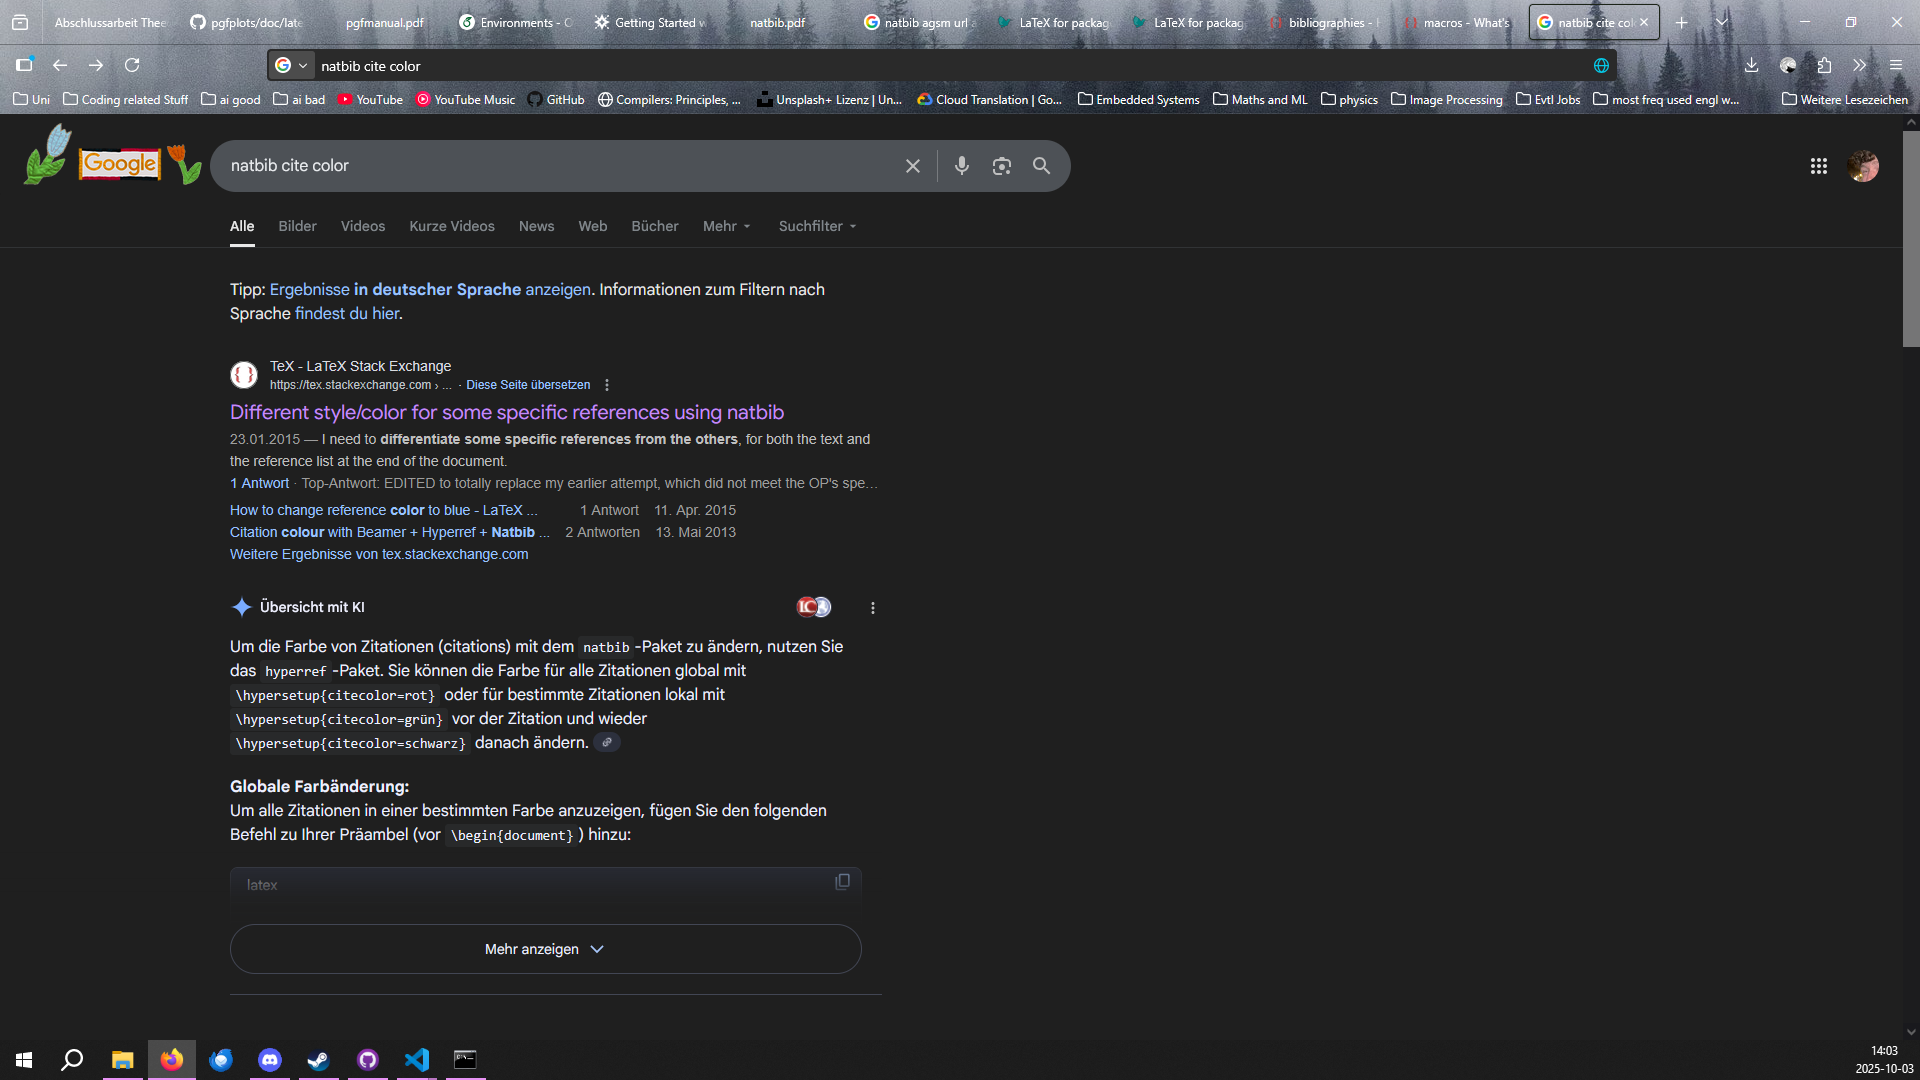
\includegraphics[width=\textwidth]{pictures/motivation.PNG}\label{fig:googlemakesmistakes}
\end{figure}
\endgroup

\end{document}